\reportsection{Cost}
\label{sec:cost}

\paragraph{What the benchmarks measure.}
The rule says which configurations support a security claim, and the benchmarks say what
those configurations cost.  Each plot fixes a binary tree with $4{,}096$ leaves and $32$
openings and reports mean prover time, verifier time, and proof size.  A field-coloured
line marks the first configuration reaching $\secpar\ge128$, and a red \textsf{x} marks
each cost transition.

\paragraph{The salt arrives in the hash's native unit.}
The rule reports the salt in the hash's own unit, $k$ field elements for an algebraic hash
such as Poseidon2~\cite{GKS23}, or $S$ bytes for a byte-oriented hash such as
Blake3~\cite{BLAKE3}.  Because the unit already matches the hash, the salt pays no encoding
penalty when it is absorbed.

\paragraph{Permutations set the transitions.}
Sponge-based hash functions operate on a \textit{state} of size $t=\text{rate}+\text{capacity}$,
where the capacity carries the previous round's output and the rate is the room left to
absorb new input.  We measure how many elements a construction absorbs before it needs a
second permutation, then overlay the security the rule certifies to mark where each field
reaches the target.

%% Measured cost of the first Poseidon2 configuration reaching lambda >= 128
%% per field and per property.  Source: ark-mt security_parameters benchmark
%% (benchmark_matrix.csv); binary tree, 4,096 leaves, 32 openings.
\begin{table}[t]
  \centering
  \small
  \begin{tabular}{llrrrr}
    \toprule
    Property & Field & Parameter & Prover (ms) & Verifier (ms) & Proof (kB) \\
    \midrule
    Hiding  & BabyBear   & $k=5$ & $25.7$  & $1.03$  & $3.6$  \\
    Hiding  & Goldilocks & $k=3$ & $39.8$  & $1.51$  & $4.6$  \\
    Hiding  & BN254      & $k=1$ & $175.2$ & $6.56$  & $10.3$ \\
    \addlinespace
    Binding & BabyBear   & $D=9$ & $38.7$  & $1.84$  & $10.1$ \\
    Binding & Goldilocks & $D=5$ & $40.3$  & $1.37$  & $11.0$ \\
    Binding & BN254      & $D=2$ & $260.0$ & $11.26$ & $16.4$ \\
    \bottomrule
  \end{tabular}
  \caption{Measured cost of the first Poseidon2 configuration reaching
  $\secpar\ge128$ per field, for the hiding benchmarks (varying the salt
  cardinality $k$) and the binding benchmarks (varying the digest width $D$).
  Prover time is mean commit plus open;
  verifier time is mean check; proof size is the compressed proof.  Fixed
  regime as in \cref{fig:poseidon-cost}: binary tree, $4{,}096$ leaves, $32$
  openings.}
  \label{tab:cost-at-128}
\end{table}


\begin{figure}[t]
  \centering
  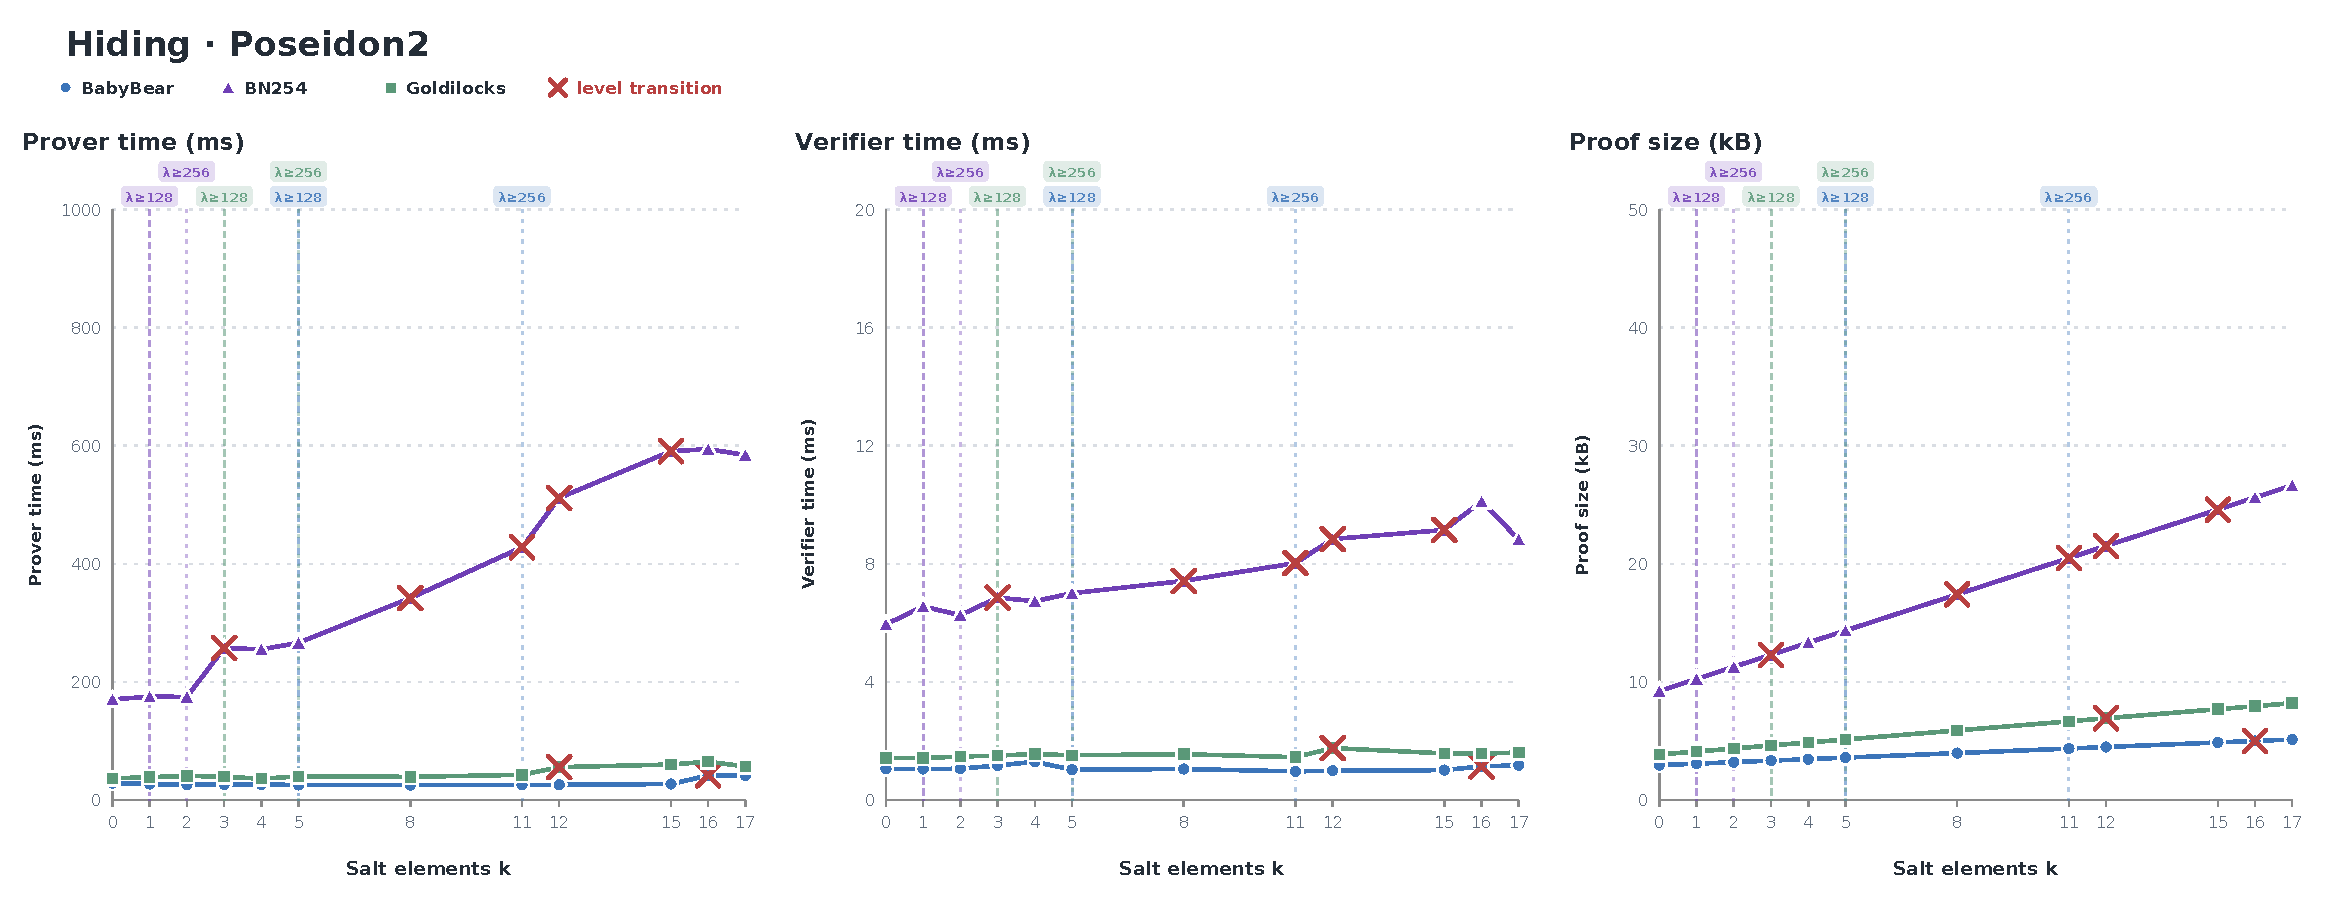
\includegraphics[width=\linewidth]{figures/benchmark_hiding_poseidon_triptych_extra_x.pdf}\\[5pt]
  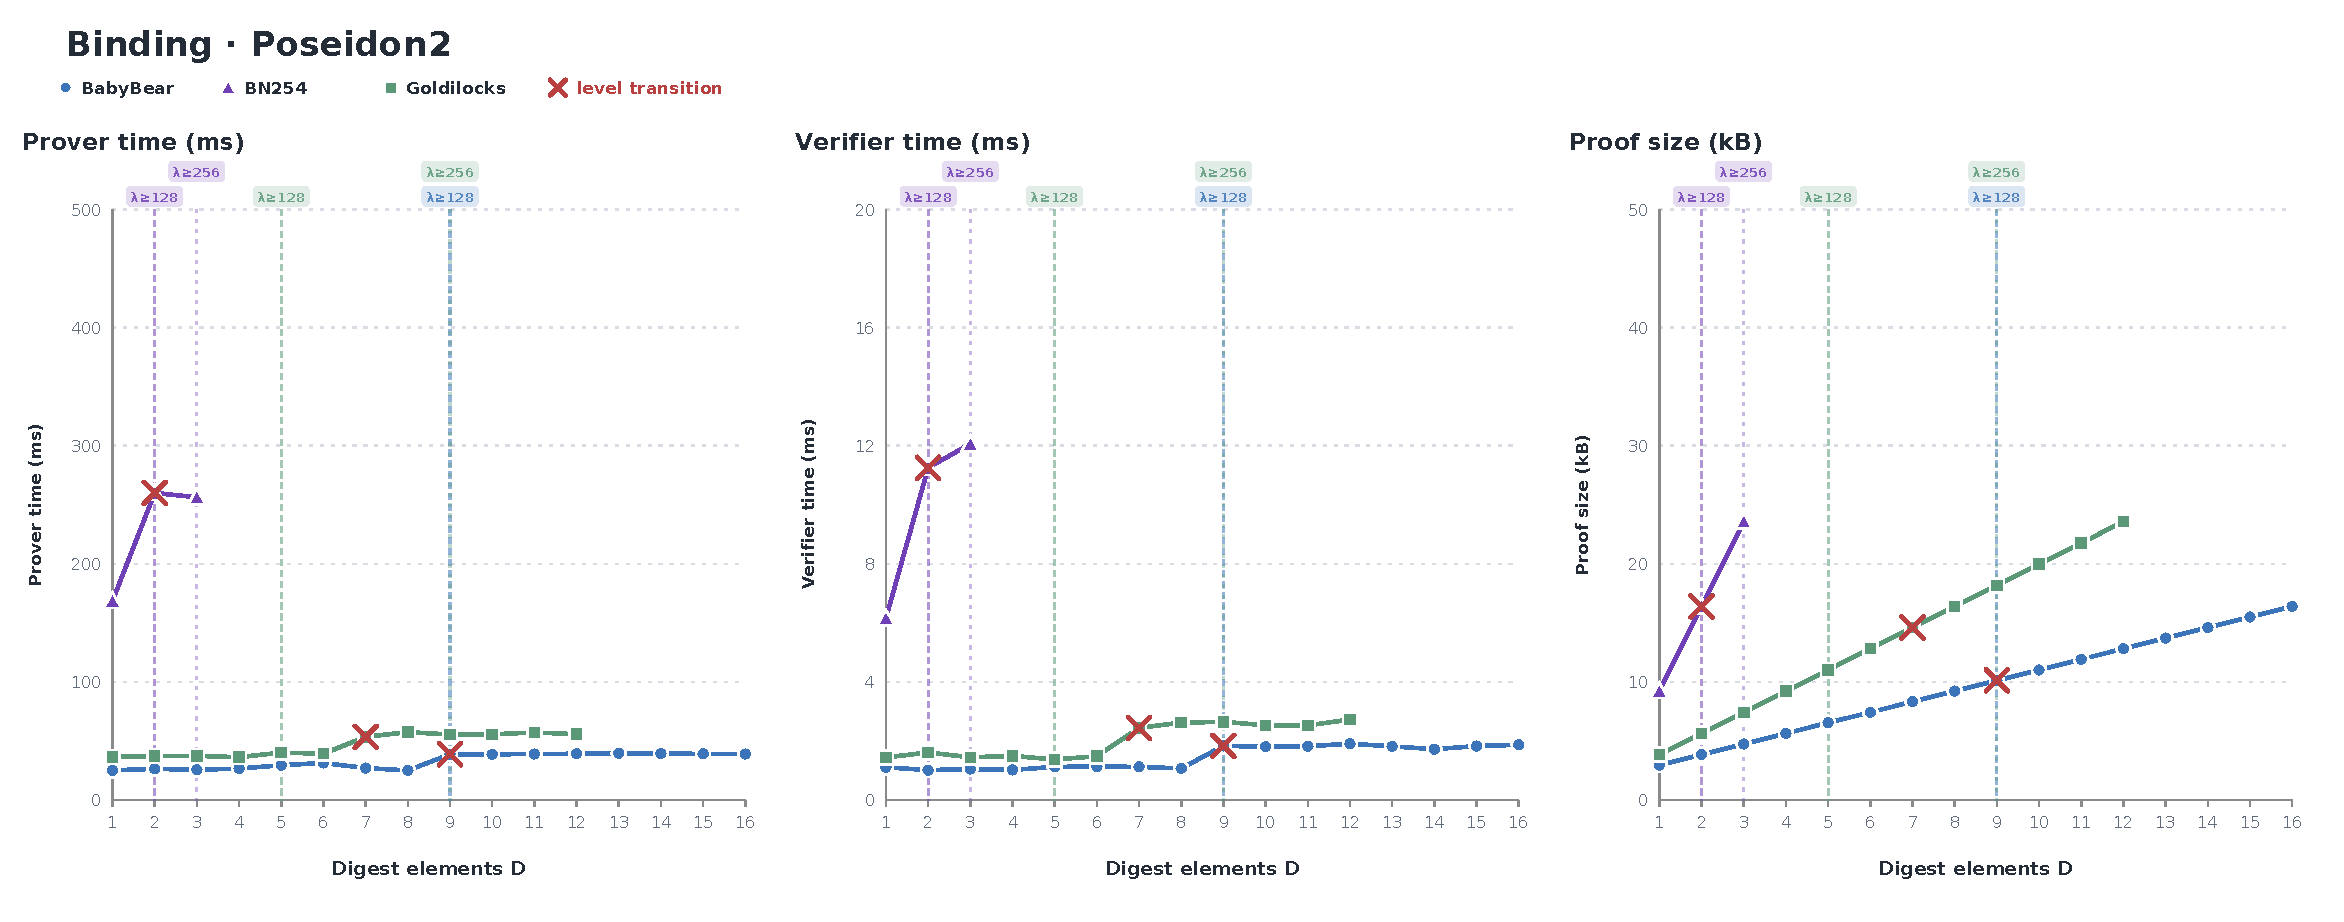
\includegraphics[width=\linewidth]{figures/benchmark_binding_poseidon_triptych_extra_x.pdf}
  \caption{Poseidon2 hiding cost as salt width grows (top) and binding cost as
  digest width grows (bottom).  Field-coloured lines mark the first measured
  $\secpar\ge128$ point for BabyBear, Goldilocks, and BN254.
  Red \textsf{x} markers flag inputs that cross into an extra permutation.}
  \label{fig:poseidon-cost}
\end{figure}

\paragraph{When binding is free.}
Proof size grows linearly with the digest width for every field, so a user with proof size
concerns can read off how much security a given size buys.  Timing has a step shape
instead: within a permutation level, widening the digest gains security at no measurable
cost, and crossing a level raises prover and verifier time sharply before flattening again.
A parent hash absorbs two child digests, so a digest is charged once per tree level while a
salt is absorbed once at the leaf, which is why a binary tree stays inside one permutation
only while $2D\le t$.  BabyBear's Poseidon2 preset runs at $t=16$ ($D\le8$ free) against a
certified $D=9$, and BN254 runs at $t=3$ ($D\le1$ free) against a certified $D=2$: both sit
one element past the boundary and pay for a second permutation, taking prover time from
$25.1$ to $38.7$~ms for BabyBear and $168.6$ to $260.0$~ms for BN254.  Goldilocks is the
exception: its $t=12$ preset holds $D\le6$ while the rule asks for only $D=5$, so its
certified binding parameters sit inside a permutation block computed anyway
(\cref{fig:hash-blocks}, left).  Proof size orders the fields the other way: Goldilocks
reaches $\secpar=128$ at fewer digest-width increments than BabyBear, yet its proof at the
crossing is the larger of the two, $11.0$ against $10.1$~kB, because each Goldilocks
element is wider.

\paragraph{Hiding is cheap everywhere.}
The rule asks for $k=5$ field salts on BabyBear, $k=3$ on Goldilocks, and $k=1$ on BN254,
while the measured leaf transitions fall at $k=16$, $k=12$, and $k=3$ respectively.  Every
field therefore reaches $\secpar=128$ well inside its first permutation block, and prover
and verifier time stay flat as the salt widens.  A user weighing hiding needs to consider
only the proof size trade-off, which grows linearly in the number of salt elements.

\paragraph{Bytewise hashers step at block boundaries.}
Blake3 compresses over fixed blocks, and an input that crosses a boundary needs a second
compression call.  Binding shows the same step structure as Poseidon2: the $\secpar=128$
digest occupies $33$ bytes, the first boundary, and crossing it takes prover time from
$1.72$ to $2.28$~ms (\cref{fig:hash-blocks}, right).  Hiding clears its own target before
the first transition, so its only cost is the proof size, which grows linearly with the
salt width.\footnote{The full bytewise Blake3 benchmark results are plotted in
\cref{fig:blake3-cost} (\cref{app:bytewise-cost}).  The prose here summarises their
result.}
\status{empirical; binary tree, $4{,}096$ leaves, $32$ openings}
